% !TEX TS-program = pdflatex
% !TEX encoding = UTF-8 Unicode

\documentclass[11pt]{article} % use larger type; default would be 10pt

\usepackage[utf8]{inputenc} % set input encoding (not needed with XeLaTeX)

%%% PAGE DIMENSIONS
\usepackage{geometry} % See geometry.pdf to learn the layout options. There are lots.
\geometry{a4paper} % or letterpaper (US) or a5paper or....

\usepackage{graphicx} % support the \includegraphics command and options

%%% PACKAGES
\usepackage{amsmath,amssymb,MnSymbol,mathrsfs}
\usepackage{enumitem}
\usepackage{float,subcaption}
\usepackage[noabbrev]{cleveref}
\usepackage{tikz}
\usepackage{amsthm}
\usepackage{bussproofs}
\usepackage{qtree}

\newtheorem{thm}{Theorem}
    \crefname{thm}{thm.}{thms.}
\theoremstyle{definition}
\newtheorem{dfn}{Definition}
    \crefname{dfn}{def.}{defs.}
    \newtheorem{subdfn}{\indent}[dfn]
    \renewcommand{\thesubdfn}{\thedfn\alph{subdfn}}
\newtheorem*{ntn}{Notation}

\newcommand{\fn}{\lambda\:\!}
\newcommand{\Ell}{\mathscr{L}}

\makeatletter
\def\rightharpoonupfill@{\arrowfill@\relbar\relbar\rightharpoonup}
\newcommand{\harpvec}{%
   \mathpalette{\overarrow@\rightharpoonupfill@}}
\makeatother

\title{A Graphical Theory of Binding}
\author{Eric Demko}
%\date{} % Activate to display a given date or no date (if empty), otherwise the current date is printed 

\begin{document}
\maketitle

\section*{What do I want out of this paper?}

All the ABT definitions I've seen aren't directly applicable to programming languages: a real language must first be ``desugared'' (a.k.a. compiled) into a form suitable for analysis by ABT.
Additionally, many formulations jump straight into category theory, which I think is a bit like smacking a fly with a sledgehammer.
There are also nameless representations, but these don't display the intuition of binding (besides: HOAS requires a pre-existing calculus, De Bruijn indices are super tedious to work with, and the Barendregt convention is unstable under usual substitution rules).
In comparison, syntax trees are super easy to work with.

I think a binding tree is just a syntax tree with some extra data describing which names are usages, which are definitions, and which names fall together.
We already have a friendly\footnote{rigorous, intuitive, hand-computable} theory (parsers) taking strings to abstract syntax trees, and I think we should have a similarly friendly theory for binding.
I think that whenever a type system or static analysis dependent on binding structure may be presented in terms of the source language directly, then the binding trees should also be in terms of the source language. More aphoristically: \emph{No compilation in the frontend}.
Such a discipline should make it easier to present compilation errors to the user in terms of their own program.

The description of ABTs I present here should make a number of things obvious from a diagram:
\begin{itemize}
    \item free variables (binding vertices with only incoming edges)
    \item unused variables (binding vertices with only an outgoing edge)
    \item alpha-renaming (pick a binding vertex and recolor all binding-edge-connected vertices (either direction) uniformly)
    \item hygienic substitution (pick a free variable and replace all usages with another graph; unify binding vertices from the two graphs according to some rule, as long as unified vertices have the name name)
    \item contexts (allow one appearance of $\square$ as a vertex in the syntax tree, which can have multiple (colored) outgoing binding edges)
    \item one-step contexts (a context where the path to $\square$ is exactly one edge long)
    \item variables bound by a context (binding vertices with an incoming edge from $\square$)
    \item hygienic substitution into an environment (replace $\square$ with the subterm's AST; link free variables of the subterm with variables bound by the context)
\end{itemize}

The theory presented here should allow a small advancement in a few areas.
Programming language specifications may now use a rigorous but clear and concise description of binding structures, akin to how they already use BNF (and extensions) to describe concrete syntax.
This theory is more accessible to computer science students than category-theoretic descriptions of binding.
It should serve as another basis for the scope analysis of compiler-compilers, and one which is particularly amenable to implementation.


\part{Intuition}

If an AST is tree-like, then a ABT is graph like: after all, you can take an AST and draw lines from variable uses to their definitions.
Exactly what a ``line'' is remains to be seen.

Note that an arity could just as well be notated as a graph fragment. For example, the arity for a lambda $A(\mathrm{lam}) = \langle e, \{\mathrm{param} \mapsto x, \mathrm{body} \mapsto e\} \rangle$ could be drawn:
\begin{center}
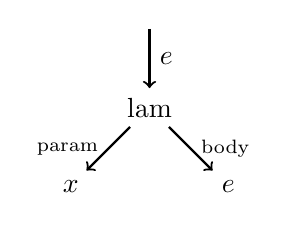
\begin{tikzpicture}
\node(op) at (0, 0) {lam};
\node(x) at (-1,-1) {$x$};
\node(e) at (1,-1) {$e$};
\draw[thick, ->] (0, 1) -- node[right] {$\scriptsize e$} (op);
\draw[thick, ->] (op) -- node[left]  {\scriptsize param} (x);
\draw[thick, ->] (op) -- node[right] {\scriptsize body}  (e);
\end{tikzpicture}
\end{center}
Grammaticality then, means that it must be possible to cover all vertices with their arities such that those arities fit together.

Since variables might be free or unused, if ``lines'' were simple edges, then one couldn't identify variables by edges alone.
Instead, let's add another vertex for each name (regardless or its being used or free), and only draw out ``lines'' through them.
(That is, the ``lines'' denoting binding are two-step paths through a special vertex.)

\part{Math}

\section{Abstract Syntax Trees}

\begin{dfn}
An abstract syntax tree (AST) $G$ is a finite arborescence\footnote{a directed rooted tree where all edges point away from the root (conventionally considered ``downwards'')} with vertices colored from a set of operators $\mathcal{O}$ and edges colored by labels $\mathcal{L}$, where for each vertex, each outwards edge must have a unique label.
\end{dfn}

It is convenient, though not necessary, to give an ordering on labels relative to each operator.
This way, the AST becomes an ordered tree, which is convenient for diagrams since the labels may be elided without ambiguity.
If the AST is the result of parsing by a context-free concrete grammar, the obvious order is that of the non-terminals in that grammar.

\begin{ntn}
Let $G$ be an AST.
We write $\overset{\downarrow}G$ to stand for the root of $G$, or $\overset{\downarrow}v \in G$ to mean that $v$ is the root of $G$.
We write $v \in G$ to mean the graph has the vertex $v$, and $\mathsf{col}(v)$ for the color of $v$
We write $v \overset{\ell}\to v' \in G$ to mean the graph has a directed edge from $v$ to $v'$ labeled $\ell$, but where the label is irrelevant, we omit the overset $\ell$.
For concision, we will omit the ``$\in G$'' where there is no ambiguity.
If $v \in G$ and $v \overset{\ell}\to v'$, then we say the child of $v$ by $\ell$ is $v'$, and since $v$ and $\ell$ uniquely identify $v'$, we can write $\ell(v) = v'$ as if each label were a function over vertices.
\end{ntn}

\begin{dfn}
We say that $p = [\harpvec{\ell_i}]$ is a path from $v_0$ to $v_n$, written $v_0 \overset{p}\twoheadrightarrow v_n$, exactly when $v \overset{\ell_i}\to v_i$ for all $1 \leq i \leq n$.
Note that $p$ may be empty; to be clear, an empty path always and only exists from a vertex to itself.
\end{dfn}

\begin{ntn}
When the path is irrelevant, we may omit it.
When $\overset{\downarrow}G \overset{p}\twoheadrightarrow v$, we may simply say that $G$ has a path to $v$ through $p$.
Every vertex $v \in G$ has a unique path from the root, so we may speak of the path to $v$.
\end{ntn}

\section{Abstract Grammar}

\begin{dfn}
Let sorts $\mathcal{S}$ be a finite set.
\begin{subdfn}
An arity is a pair $\langle s_\uparrow, \{\harpvec{\ell \mapsto s_\downarrow}\} \rangle$, where $s_\uparrow$ is a sort called the upwards arity, and $\{\harpvec{\ell \mapsto s_\downarrow}\}$ is a finite map from labels to sorts called the ``downwards arity''.
\end{subdfn}
\begin{subdfn}
An abstract grammar is a pair $\langle s_0, A \rangle$, where $s_0 \in \mathcal{S}$ is called the start sort, and $A$ is  an arity function mapping operators to arities.
\end{subdfn}
\end{dfn}

\begin{ntn}
We will often have need of the upwards- and downwards-arity separately; whenever $A(o) = \langle s_\uparrow, \harpvec{\ell \mapsto s_\downarrow} \rangle$, we will write $A_\uparrow(o) = s_\uparrow$ and $A_\downarrow(o) = \harpvec{\ell \mapsto s_\downarrow}$.
Recall that we will pass vertices where operators are expected; $A, A_\uparrow, A_\downarrow$ will often be used in this way.
Also, we will say ``the sort of a vertex'' to mean ``the upwards-arity of the operator coloring a vertex''.
We will often need to enumerate the outgoing edge labels for an operator; for this, we will use the function $\Ell(o) = \mathsf{dom}(A_\downarrow(o))$.
\end{ntn}

\begin{dfn}
An AST $G$ is grammatical w.r.t. an abstract grammar $\langle s_0, A \rangle$ iff:
\begin{enumerate}[label=\alph*)]
\item The sort of the root must be the start sort $A_\uparrow(\overset{\downarrow}G) = s_0$, and
\item every vertex, for each label in its downwards arity, must have a child by that label whose sort is given by the arity.
    $$\forall v \in G, \langle \ell \mapsto s' \rangle \in A_\downarrow(v).\, \exists v'.\,v \overset{\ell}\to v' \land \mathsf{col}(v') = s'$$
\end{enumerate}
\end{dfn}


\section{Abstract Binding Trees}

\begin{dfn}
Let $\mathcal{N}$ be a set of names.
Operators may be parameterized by at most one name, in which case we say that the operator ``has a name''.
When an operator $o$ is parameterized by a name $x$, we write $\mathsf{name}(o) = x$.
\end{dfn}

\begin{dfn}
\label{def:abt}
An abstract binding tree (ABT) is a graph where both vertices and edges can be partitioned into two types, syntactic and binding, subject to the following restrictions:
\begin{enumerate}[label=\alph*)]
\item The subgraph which contains only syntactic vertices and edges is an AST.
\item Each non-empty maximal binding-edge-connected subgraph is a star graph,
        rooted at a binding edge,
        where all of the leaves are syntactic and share the same name, and
        the leaves with root-wards edges share the same sort.
\end{enumerate}
Note that, although syntactic edges and nodes are colored, binding nodes and edges need not be.
(NOTE: There isn't at most binder for a variable, b/c of stuff like $\{e:\alpha + \alpha\} \vdash \mathsf{case}\;e\;\mathsf{of}\;\{\iota_1\;x \mid \iota_2\;x \Rightarrow x\}:: \alpha$.)
\begin{subdfn}
Further, two ABTs are equivalent if they differ only by disconnected binding vertices.
\end{subdfn}
\begin{subdfn}
A proper ABT is connected, and is therefore the unique minimal graph in said equivalence set.
\end{subdfn}
\end{dfn}

\begin{ntn}
Let $G$ be an ABT.
When we write $v \in G$, we make no distinction between syntactic and binding vertices; we write $\mathsf{syn}(G)$, $\mathsf{var}(G)$ respectively for the syntactic and binding vertices.
We use the same notations from before to refer to the syntactic root ($\overset{\downarrow}G$) and the existence of syntactic edges ($v \overset{\ell}\to v' \in G$).
When there is a binding edge from $v$ to $v'$, we write $v \dashedrightarrow v' \in G$.
\end{ntn}

\begin{dfn}
We say that $p$ is a path from $v_0$ to $v_n$, written $v_0 \overset{p}\twoheadrightarrow v_n$.
Unlike the notation for ASTs, $p$ may take one of three forms.
If $p = [\harpvec{\ell_i}]$, then the definition is as for ASTs.
If $p = [\harpvec{\ell_i},{\dashedrightarrow}]$, then the path exists exactly when $v \overset{\ell_i}\to v_i$ for all $1 \leq i \leq n-1$, and $v_{n-1} \dashedrightarrow v_n$.
Similarly, if $p = [\harpvec{\ell_i},{\dashedleftarrow}]$, then the path exists exactly when $v \overset{\ell_i}\to v_i$ for all $1 \leq i \leq n-1$, and $v_n \dashedrightarrow v_{n-1}$.
\end{dfn}

\begin{ntn}
When the path is irrelevant, we may omit it.
When $\overset{\downarrow}G \overset{p}\twoheadrightarrow v$, we may simply say that $G$ has a path to $v$ through $p$.
Every vertex $v \in G$ which is not a weakening variable has a path from the root, so we may speak of the paths to $v$.
\end{ntn}

\begin{dfn}
If $G$ is an ABT, then its scope erasure $\mathsf{noscope}(G)$ is an AST that contains exactly the syntactic vertices and edges from $G$.
Note that the scope erasure is exactly the subgraph mentioned in \cref{def:abt}a.
\end{dfn}

\begin{dfn}
A variable is a non-empty maximal binding-edge connected subgraph of an AST.
Note that variables are exactly the subgraphs mentioned in \cref{def:abt}b.
\end{dfn}

\begin{dfn}
A usage of a variable is a syntactic vertex in that variable with an outgoing binding edge.
These are exactly the leaves of variables with root-wards edges mentioned in \cref{def:abt}b.
\end{dfn}

\begin{dfn}
A binder of a variable is a syntactic vertex in that variable with an incoming binding edge.
\end{dfn}

\begin{ntn}
Since each variable has a unique binding vertex $v$ at its center, we will equivocate between variables and binding vertices where this will not cause confusion.
Since all of the syntactic vertices in a variable have the same name, it is sensible to say that a variable has a name, which we write $\mathsf{name}(v) = x$.
\end{ntn}

\section{Free Variables, and other properties of variables}

\begin{dfn}
Variables may have certain notable properties:
\begin{subdfn}
A free variable is one which has no binder.
Variables which are not free are called bound variables.
\end{subdfn}
\begin{subdfn}
An unused variable is one which has no usage.
Variables which are not unused are called used variables.
\end{subdfn}
\begin{subdfn}
A weakening variable is one with no binding edges at all, or equivalently a variable both free and unused.\footnote{By definition, these cannot occur in a proper ABT, but are useful to simplify certain definitions and theorems later; however they are generally uninteresting in applications.}
Variables which are not weakening are called proper variables.
\end{subdfn}
\end{dfn}

\begin{dfn}
Let $G$ be an ABT, then $\mathsf{fv}(G)$ is the set of all free, used variables in $G$.
\end{dfn}

There's something very pleasant about this definition of free variables.
It's quite natural (assuming our ABTs seem natural to you), but more importantly, it is applicable to any language with binding.
Existing definitions of $\mathsf{fv}$ in the literature are usually ad-hoc only and for a single language.

\begin{dfn}
Let $G, G', F$ be distinct ABTs.
\begin{subdfn}
    We say that $v \in G$ has a copy $\dot v \in G'$, written $\mathsf{copy}(v) = \dot v$ exactly when
    for every path to $v$ in $G$, the same path in $G'$ leads to $\dot v$,
    $\dot v$ is syntactic iff $v$ is, and
    (if applicable) $\mathsf{col}(v) = \mathsf{col}(\dot v)$.
\end{subdfn}
\begin{subdfn}
    We say that a vertex $w \in F$ has a copy $\dot w_u \in G'$ by $u \in G$, written $\mathsf{copy}_u(w) = \dot w_u$ exactly when
    for every path $p$ to $u$ in $G$ and path $p'$ to $w$ in $F$, the path $p,p'$ in $G'$ leads to $\dot w_u$,
    $\dot w_u$ is syntactic iff $w$ is, and
    (if applicable) $\mathsf{col}(w) = \mathsf{col}(\dot w_u)$.
\end{subdfn}
\end{dfn}

\begin{ntn}
Where there is a unique copy $\dot v = \mathsf{copy}(v)$, we may write $\mathsf{copy}(v)$ for $\dot v$.
We say that an ABT $G'$ contains a copy of $G$, written $\mathsf{copy}(G) \in G'$, when there is a distinct copy in $G'$ of every vertex in $G$.
Similarly, an ABT $G'$ contains a copy of $F$ at $u \in G$, written $\mathsf{copy}_u(F) \in G'$, when there is a distinct copy by $u$ in $G'$ of every vertex in $F$.
\end{ntn}

TODO: Note/lemma: if $\dot F = \mathsf{copy}_u(F) \in G'$ and $\dot F' = \mathsf{copy}_{u'}(F) \in G'$ for distinct $u,u'$, then $\dot F, \dot F'$ are disjoint.
This is b/c the sets of paths to $u, u'$ are disjoint.


\section{Renaming}

\begin{dfn}
Name-parameterized operators have a natural relationship, renaming, which we write $o[\mapsto y]$.
Where the operator is known to have the name $x$, as in $o[x]$, then $o[x][\mapsto y] = o[y]$.
Where the operator is known not to have a name, as in $o$, then $o[\mapsto y] = o$.
\end{dfn}

\begin{dfn}
When $G$ is an ABT and $v$ is a variable in $G$, we write $G[v \mapsto y]$ for the graph with $v$ renamed to $y$.
That graph is identical to $G$, except that all syntactic vertices in the variable\footnote{``in the variable'' $\equiv$ ''connected to the binding vertex''} $v$ are renamed to $y$.
\end{dfn}

\begin{ntn}
When multiple variables are to be renamed, as in $G[v_1 \mapsto x_1]\ldots[v_n \mapsto x_n]$, we may write $G' = G[v_1 \mapsto x_1, \ldots, v_n \mapsto x_n]$ where $v_1,\ldots,v_n$ are distinct.
\end{ntn}

\begin{dfn}
Two ABTs $G, G'$ are $\alpha$-equivalent when one may be obtained from the other by renaming zero or more \emph{bound} variables.
\end{dfn}

\begin{ntn}
Wherever two ABTs are $\alpha$-equivalent, we say that one may $\alpha$-rename (a.k.a. $\alpha$-convert) one into the other.
It is often useful in applications to consider the set of ABTs modulo $\alpha$-equivalence, or equivalently to say ABTs are identical up to $\alpha$-renaming.
During static analysis or debugging however, it is better not to alter names, since they serve as useful guideposts to programmers.
\end{ntn}

Normally, $\alpha$-renaming is defined in terms of substitution, but obviously we haven't yet introduced substitution.
Under the graphical formulation of ABTs, $\alpha$-renaming and substitution may be defined separately, which I think is an interesting bit of analysis.

\begin{thm}
\label{thm:unique-names}
For every ABT, there is an $\alpha$-equivalent ABT where each bound variable has a distinct name also distinct from the names of any free variables, as long as $\mathcal{N}$ has a sufficient supply of names.
\end{thm}

\begin{thm}
\label{thm:singleton-names}
For every ABT, there is an $\alpha$-equivalent ABT where each bound variable has the same name.
In this context, we can simply elide the names of bound variables altogether.
\end{thm}

Use of the Barendregt convention takes advantage of \cref{thm:unique-names} in contexts where ABTs modulo $\alpha$-renaming are studied.
Similarly, De Bruijn indices and other nameless representations are motivated by \cref{thm:singleton-names}.
For De Bruijn indices, each index is in fact a description of the syntactic path from a variable usage to a variable binder such that the path through binding edges has the same endpoint.


\section{Substitution}

\begin{dfn}
Substitution $[v \mapsto G'; \harpvec{v_i \sim v'_i}]G$ replaces usages of a free variable $v$ in $G$ with copies of $G'$, except the binding vertices of free variables are merged in one of two ways.
The copy of each $y_i$ includes not only usages from $G$, but also usages from all copies of $F$;
the other free variables of $F$ each have usages from all copies of the original usages.

More precisely, let $F, G$ be ABTs, $x$ be a free variable in $G$, $\harpvec{y_i}$ be distinct free variables in $G$ also distinct from $x$, and $\harpvec{y'_i}$ be distinct free variables in $F$, with $\mathsf{name}(y_i) = \mathsf{name}(y'_i)$ and $\mathsf{sort}(y_i) = \mathsf{sort}(y'_i)$.
Then $[x \mapsto F; \harpvec{y_i \sim y'_i}]G = G'$ if $G'$ is the smallest ABT such that all of the following are satisfied:
\begin{enumerate}[label=\alph*)]
\item $G'$ contains a copy of $G$ except for the variable $x$.
    $$\mathsf{copy}(G-x) \in G'$$
\item Let $f = F - \bigcup_{x' \in \mathsf{fv}(F)}\mathsf{var}(x')$, which is the syntactic part of $F$ along with all its bound variables, but none of the binding vertices of its free variables.
    Then $G'$ contains a (distinct) copy of $f$ for each usage of $x$.
    $$\forall u \in \mathsf{syn}(x).\, \mathsf{copy}_u(f) \in G'$$
    Note that, since $x$ is free, $\mathsf{syn}(x)$ contains exactly the usages of $x$.
\item Whenever $F$ uses a variable $y'_i$ where $y_i \sim y'_i$, its copies in $G'$ are instead usages of $y_i$.
    $$\forall w \dashedrightarrow y'_i \in F.\,
        \forall u \in \mathsf{syn}(x).\,
        \mathsf{copy}_u(w) \dashedrightarrow \mathsf{copy}(y_i) \in G'$$
\item For each of the other free variables of $F$, there is a corresponding free variable in $G'$ whose usages are exactly the copies of its usages in $F$.
    \begin{align*}
    & \forall x' \in \mathsf{fv}(F) - \{\harpvec{y'_i}\}.\,
        \exists \dot x' \in \mathsf{fv}(G'). \\
    &\quad \forall w \in F,
        u \in \mathsf{syn}(x),
        \dot w_u = \mathsf{copy}_u(w) \in G'. \\
    & \quad\qquad
            \dot w_u \dashedrightarrow \dot x' \Leftrightarrow w \dashedrightarrow x'
    \end{align*}
\end{enumerate}
\end{dfn}

\begin{ntn}
When multiple variables are to be substituted for, as in $G[v_1 \mapsto G'_1; \harpvec{v_i \sim v'_i}]\ldots[v_n \mapsto G'_n; \harpvec{v_i \sim v'_i}]G$, we may write $G[v_1 \mapsto G_1, \ldots, v_n \mapsto G_n; \harpvec{v_i \sim v'_i}]$ where $v_1,\ldots,v_n$ are distinct.\footnote{note that all $\harpvec{v_i \sim v'_i}$ are identical}
Where it is obvious (usually, where $G, G'$ are both derived from the same ABT), we may omit the $\harpvec{v_i \sim v'_i}$.
\end{ntn}


\section{Hygiene}

\begin{dfn}
Let $G, G'$ be ABTs, $v \in G$ be a variable and $\dot v \in G'$ a copy (either $\dot v = \mathsf{copy}(v)$ directly, or $\dot v = \mathsf{copy}_u(v)$ by some $u$).
The vertices $v, \dot v$ are said to be confused unless both of the following are true:
\begin{enumerate}[label=\alph*)]
\item The vertex $\dot v$ is free/bound exactly when $v$ is.
\item For each distinct $v' \in G$ with a copy $\dot v' \in G'$ (again, either directly or by some $u'$), $\dot v, \dot v'$ are distinct.
\end{enumerate}
\end{dfn}


\begin{thm}
\label{thm:no-confusion}
The operations of $\alpha$-renaming and substitution do not (accidentally) confuse variables.
That is:
\begin{description}%[label=\alph*)]
\item[For $\alpha$-renaming] No variable in $G$ is confused with any variable in $[v \to y]G$.
\item[For substitution] The variables confused between $G, F$ on the one hand and\newline$[x \to F; \harpvec{y_i \sim y'_i}]G$ on the other are exactly $y_i$ with $y'_i$.
\end{description}
\end{thm}

With \cref{thm:no-confusion}, we have a remarkable result:
substitution and $\alpha$-renaming are \emph{always} hygienic in this formulation of binding, regardless of the language we are working in, or even if the ABTs we are operating on are grammatical!
As long as we limit ourselves to these operations, which is hardly a limitation at all, variables will never get confused with one another.
Even through all this, our ABTs nevertheless are direct representations of the source code, which allows us to more easily report compilation errors or include debugging symbols, and thus supporting our mantra \emph{no compilation in the frontend}.

In contrast, a carefully-defined hygienic substitution operator is only applicable to a single formal language.
De Bruijn indices are again only useful in a single language, and must be generalized to account for even slightly more complex binding structures, such as pattern-matching.\footnote{Admittedly, such a generalization of De Bruijn indices is a natural match with our accounting of bound variables. Our theory is strictly more powerful when it comes to free variables, however.}
Barendregt's variable convention is usable across languages, but is unstable under substitution.\footnote{variables must be made unique again after each substitution, not just initially}
Thus, even though \cref{thm:unique-names,thm:singleton-names} justify these techniques, we will not have need of them.


\section*{MORE STUFF}

TODO: binding grammar

TODO: (earlier) sub-grammar.
TODO: since all usages of a binding vertex have the same sort, the sort of that binding vertex is the sort of its usages.
TODO: if $G$ is grammatical, and $F$ is grammatical w.r.t. the subgrammer on $s$, then $[x \mapsto F; \harpvec{y_i \sim y'_i}]G$ is grammatical

TODO: our notions of $\mathsf{fv}$, renaming, ans substitution coincide with the usual definitions on logics, the lambda calculus and its common variants, the pi calculus and its common variants, and so on

TODO ``context-free'' only bind a usage to the closest of its scoping parents; ``context-sensitive'' only bind a usage to binders when they share a common ancestor which scopes over the usage.
These might need contexts to define as well.

TODO: there must be a relationship between $\alpha$-renaming and substitution, but since $\alpha$-renaming operates on bound variables and substitution on free, I think I'll need contexts defined first.

\part{Notes}

TODO: I might like to define notions of copying vertices. That'd make a very formal description of $\alpha$-renaming, substitution, and confusion/hygiene much easier.
(When $G' = G[v \mapsto y]$, and $v \in G$, then the copy of $v$ in $G'$ is $\dot v \in G'$ such that...; similarly for the/a copy under substitution)
TODO: If I do that, I'd also like to mention $v \to v' \to v''$ and similar relation-like shortcuts, $v\to \to v''$ when $v'$ is not important, and $v \twoheadrightarrow v'$ for the reflexive-transitive closure of $\to$

NOTE TO SELF: usually $\alpha$-renaming is defined in terms of substitution, but here I can define them independently (though substitution preserves grammaticality, which is in turn defined in terms of $\alpha$-renaming). Since it puts $\alpha$-equivalence prior to any more complex operations on ABTs, that's quite nice: if the interesting properties of ABTs are conserved by $\alpha$-renaming, let's define $\alpha$ up front and just work in the residue from the get-go.

NOTE TO SELF: $\alpha$-renaming for bound variables, substitution for free variables; also, there's a difference between renaming and $\alpha$-renaming

FIXME: I may want to restrict ABTs so that usages of a variable share the same sort

NOTE TO SELF: it seems like a variable could be a directed hyperedge (where there's an in-set and out-set, either of which may be empty)

NOTE TO SELF: non-leaf nodes can have binding edges, such as for $\mathsf{lam}[x](\mathsf{expr})$

$$
\mathsf{case}\;x\;\mathsf{of}\;\{
    \iota_1\;(f, a) \to f\;a \:;\:
    \iota_2\;f \to f\;f
\}
$$
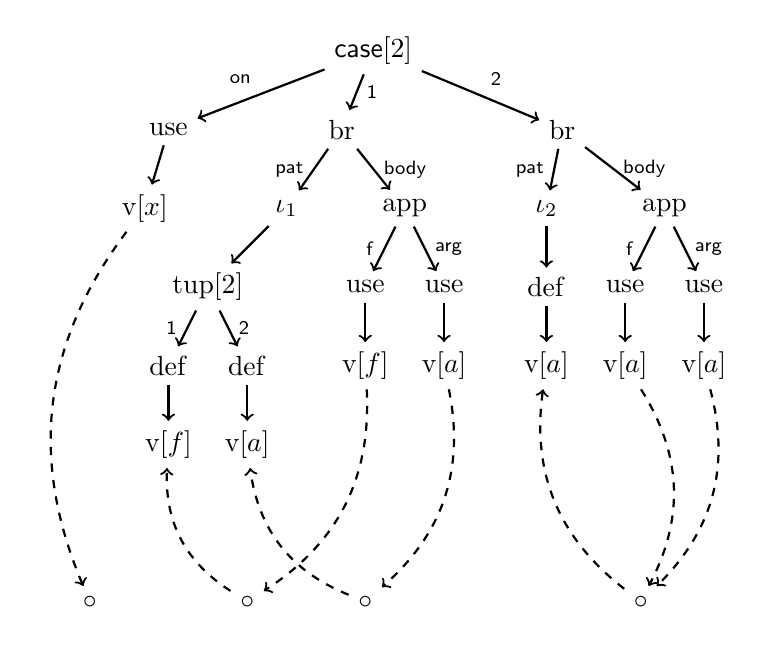
\begin{tikzpicture}
\node(r) at (1.6,0) {$\mathsf{case}[2]$};
    \node(r1) at (-1,-1) {$\mathrm{use}$};
        \node(r11) at (-1.3,-2) {$\mathrm{v}[x]$};
    \node(r2) at (1.2,-1) {$\mathrm{br}$};
        \node(r21) at (0.5,-2) {$\iota_1$};
            \node(r211) at (-0.5,-3) {$\mathrm{tup}[2]$};
                \node(r2111) at (-1,-4) {$\mathrm{def}$};
                    \node(r21111) at (-1,-5) {$\mathrm{v}[f]$};
                \node(r2112) at (0,-4) {$\mathrm{def}$};
                    \node(r21121) at (0,-5) {$\mathrm{v}[a]$};
        \node(r22) at (2,-2) {$\mathrm{app}$};
            \node(r221) at (1.5,-3) {$\mathrm{use}$};
                \node(r2211) at (1.5,-4) {$\mathrm{v}[f]$};
            \node(r222) at (2.5,-3) {$\mathrm{use}$};
                \node(r2221) at (2.5,-4) {$\mathrm{v}[a]$};
    \node(r3) at (4,-1) {$\mathrm{br}$};
        \node(r31) at (3.8,-2) {$\iota_2$};
            \node(r311) at (3.8,-3) {$\mathrm{def}$};
                \node(r3111) at (3.8,-4) {$\mathrm{v}[a]$};
        \node(r32) at (5.3,-2) {$\mathrm{app}$};
            \node(r321) at (4.8,-3) {$\mathrm{use}$};
                \node(r3211) at (4.8,-4) {$\mathrm{v}[a]$};
            \node(r322) at (5.8,-3) {$\mathrm{use}$};
                \node(r3221) at (5.8,-4) {$\mathrm{v}[a]$};

\draw [thick,->] (r)     -- node[above left]  {\scriptsize\textsf{on}}   (r1);
\draw [thick,->] (r)     -- node[right]       {\scriptsize\textsf{1}}    (r2);
\draw [thick,->] (r)     -- node[above right] {\scriptsize\textsf{2}}    (r3);
\draw [thick,->] (r1)    -- node[]            {\scriptsize\textsf{}}     (r11);
\draw [thick,->] (r2)    -- node[left]        {\scriptsize\textsf{pat}}  (r21);
\draw [thick,->] (r2)    -- node[right]       {\scriptsize\textsf{body}} (r22);
\draw [thick,->] (r21)   -- node[]            {\scriptsize\textsf{}}     (r211);
\draw [thick,->] (r211)  -- node[left]        {\scriptsize\textsf{1}}    (r2111);
\draw [thick,->] (r211)  -- node[right]       {\scriptsize\textsf{2}}    (r2112);
\draw [thick,->] (r2111) -- node[]            {\scriptsize\textsf{}}     (r21111);
\draw [thick,->] (r2112) -- node[]            {\scriptsize\textsf{}}     (r21121);
\draw [thick,->] (r22)   -- node[left]        {\scriptsize\textsf{f}}    (r221);
\draw [thick,->] (r22)   -- node[right]       {\scriptsize\textsf{arg}}  (r222);
\draw [thick,->] (r221)  -- node[]            {\scriptsize\textsf{}}     (r2211);
\draw [thick,->] (r222)  -- node[]            {\scriptsize\textsf{}}     (r2221);
\draw [thick,->] (r3)    -- node[left]        {\scriptsize\textsf{pat}}  (r31);
\draw [thick,->] (r3)    -- node[right]       {\scriptsize\textsf{body}} (r32);
\draw [thick,->] (r31)   -- node[]            {\scriptsize\textsf{}}     (r311);
\draw [thick,->] (r311)  -- node[]            {\scriptsize\textsf{}}     (r3111);
\draw [thick,->] (r32)   -- node[left]        {\scriptsize\textsf{f}}    (r321);
\draw [thick,->] (r32)   -- node[right]       {\scriptsize\textsf{arg}}  (r322);
\draw [thick,->] (r321)  -- node[]            {\scriptsize\textsf{}}     (r3211);
\draw [thick,->] (r322)  -- node[]            {\scriptsize\textsf{}}     (r3221);

\node(x) at (-2,-7) {$\circ$};
\node(f1) at (0,-7) {$\circ$};
\node(a1) at (1.5,-7) {$\circ$};
\node(a2) at (5,-7) {$\circ$};

\draw [dashed,thick,->] (r11)    to[bend right] (x);
\draw [dashed,thick,->] (f1)    to[bend left]  (r21111);
\draw [dashed,thick,->] (r2211) to[bend left]  (f1);
\draw [dashed,thick,->] (a1)    to[bend left]  (r21121);
\draw [dashed,thick,->] (r2221) to[bend left]  (a1);
\draw [dashed,thick,->] (a2)    to[bend left]  (r3111);
\draw [dashed,thick,->] (r3211) to[bend left]  (a2);
\draw [dashed,thick,->] (r3221) to[bend left]  (a2);

\end{tikzpicture}


$$(\fn x.\,e)\;e' \to [x \mapsto e']e$$
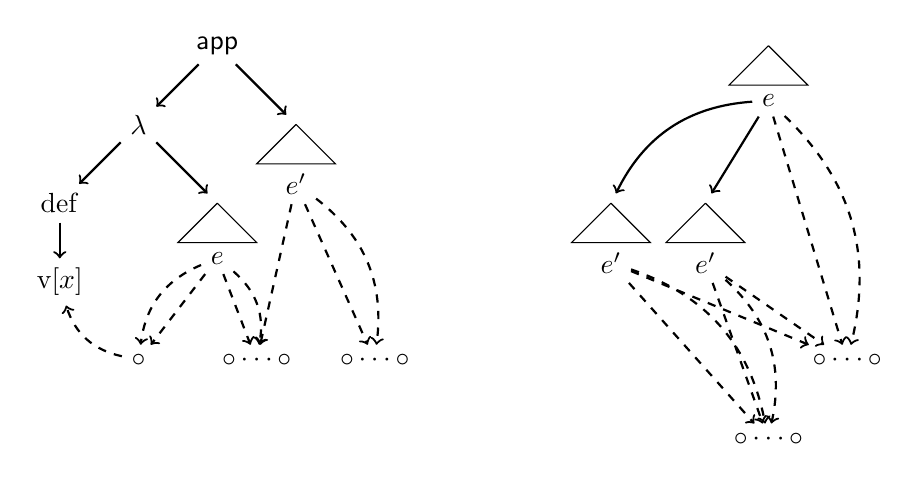
\begin{tikzpicture}
\node(r) at (0,0) {$\mathsf{app}$};
    \node(r1) at (-1,-1) {$\lambda$};
        \node(r11) at (-2,-2) {$\mathrm{def}$};
            \node(r111) at (-2,-3) {$\mathrm{v}[x]$};
        \node(r12) at (0,-2) {};
    \node(r2) at (1,-1) {};

\draw (0,-2) -- (-0.5,-2.5) -- node(e)[below] {$e$} (0.5,-2.5) -- (0,-2);
\draw (1,-1) -- (0.5,-1.5) -- node(e')[below] {$e'$} (1.5,-1.5) -- (1,-1);

\draw [thick,->] (r) -- (r1);
\draw [thick,->] (r) -- (r2);
\draw [thick,->] (r1) -- (r11);
\draw [thick,->] (r1) -- (r12);
\draw [thick,->] (r11) -- (r111);

\node(x) at (-1,-4) {$\circ$};
\node(fvs1) at (0.5,-4) {$\circ\cdots\circ$};
\node(fvs2) at (2,-4) {$\circ\cdots\circ$};

\draw[dashed,thick,->] (x) to[bend left] (r111);
\draw[dashed,thick,->] (e) to[bend right] (x);
\draw[dashed,thick,->] (e) to[] (x);
\draw[dashed,thick,->] (e) to[bend left] (fvs1);
\draw[dashed,thick,->] (e) to[] (fvs1);
\draw[dashed,thick,->] (e') to[] (fvs1);
\draw[dashed,thick,->] (e') to[] (fvs2);
\draw[dashed,thick,->] (e') to[bend left] (fvs2);


\draw (7,0) -- (6.5,-0.5) -- node(e)[below] {$e$} (7.5,-0.5) -- (7,0);
\draw (5,-2) node(e'1) {} -- (4.5,-2.5) -- node(e'1u)[below] {$e'$} (5.5,-2.5) -- (5,-2);
\draw (6.2,-2) node(e'2) {} -- (5.7,-2.5) -- node(e'2u)[below] {$e'$} (6.7,-2.5) -- (6.2,-2);

\draw[thick,->] (e) to[bend right] (e'1);
\draw[thick,->] (e) to[] (e'2);

\node(fvs1) at (8,-4) {$\circ\cdots\circ$};
\node(fvs2) at (7,-5) {$\circ\cdots\circ$};

\draw[dashed,thick,->] (e) to[] (fvs1);
\draw[dashed,thick,->] (e) to[bend left] (fvs1);
\draw[dashed,thick,->] (e'1u) to[] (fvs1);
\draw[dashed,thick,->] (e'2u) to[] (fvs1);
\draw[dashed,thick,->] (e'1u) to[] (fvs2);
\draw[dashed,thick,->] (e'2u) to[] (fvs2);
\draw[dashed,thick,->] (e'1u) to[bend left] (fvs2);
\draw[dashed,thick,->] (e'2u) to[bend left] (fvs2);

\end{tikzpicture}

The thing is, I'll need to not just replace the nodes that have binding edges out, but a subtree whose shape might often look different.
Perhaps I really do need to have names simply as parameters to nodes, and restrict binding edges to leaf nodes of a single parameter, and the parameters must match among nodes connected by binding edges.

A good example for the ease of hygiene is $(\fn x,y.\,x)\;y$. Sure, following subtitution in the graph leads to a ABT that cannot be inferred from its AST (obtained by erasure of binding vertices and edges), but after $\alpha$-renaming, erase+infer is idempotent.


\part{Draft}

\section{Introduction}

There are lots of minor variants on existing programming language calculi.
The definitions of these variants often inject only minimal changes into a formal description (See Figs. 1 and 2).
It's a shame to have to make widespread changes to an existing codebase in order to implement such extensions.

\begin{figure}[H]
\centering
    \begin{subfigure}[t]{0.3\textwidth}
        \begin{align*}
            e ::=&\; x \\
              \mid&\; \fn x.\,e \\
              \mid&\; e\;e
        \end{align*}
        \begin{align*}
            (\fn x.\,e)\;e' \longrightarrow e[x \mapsto e']
        \end{align*}

    \caption{Pure $\lambda$}
    \end{subfigure}
    \begin{subfigure}[t]{0.3\textwidth}
        \begin{align*}
            e ::=&\; \ldots \\
              \mid&\; (e_1, \ldots, e_n) \\
              \mid&\; \pi_i\;e
        \end{align*}
        \begin{align*}
            \pi_i\;(e_1, \ldots, e_n) &\longrightarrow e_i
        \end{align*}
    \caption{$\lambda$ extended with tuples}
    \end{subfigure}
\end{figure}


The informal description leaves a lot out: notions of free/bound variables, hygienic substitution, contexts, and so on as needed for various reduction rules.
All these are quite boring and could be automated, except for the binding structure, which underlies all uses of variables.
While the binding structure is intuitively obvious to humans, it would be better to present it formally so that we can debug the computer's variable-related reasoning by reference to our definitions.

Intuitively, binding is an additional layer of structure on top of an abstract grammar, and we would like to maintain that distinction.
First, we will present our target (ABTs) as an extension of what we have (ASTs); with these we can naturally define free variables, hygienic substitution, $\alpha$-conversion, and so on (collectively: variable-manipulation operations).
Then, we will describe 1) a framework for producing an ABT from an AST acording to a set of rules, and 2) a simple notation with which to present the rules.
Although this framework will not cover all languages, it should be useful for lexically-scoped functional programming languages.
We will then show that, for exemplary calculi, the obvious binding rules give rise to variable-manipulation operations identical in function to standard manipulations.

\section*{Notes}

The scope erasure of an ABT is the AST obtained by removing all binding vertices and edges.
A binding grammar is a subset of operators called name operators, an equivalence relation on name operators, and a scope analysis.
A scope analysis is a partial function from ASTs to ABTs such that binding erasure on the result yields the original AST.
An ABT is grammatical w.r.t. a binding grammar if a) all sets of syntactic vertices connected by binding edges are colored by equivalent name operators, and b) there is some $\alpha$-renaming of it for which scope analysis after binding erasure on the renamed ABT yields the renamed ABT again.
There is probably a complexity hierarchy of binding grammars (if the function is computable seems an obvious choice akin to recursively enumerable languages).


\section{A Graphical Presentation of ABTs}

Let's quickly review abstract syntax trees and abstract grammars.
The trees we will use are non-empty, finite, and are colored on both edges and labels, but otherwise are standard trees;
that is, we are concerned with graphs that have exactly one distinguished vertex, the root, which has no inwards edge, and there is a unique path to any vertex from the root.
The color of an edge or vertex $\eta$ is denoted by $\mathsf{col}(\eta)$.
If a graph $G$ has a vertex $v$, we write $v \in G$, and if it is the root, we write $\overset\downarrow v$.
If a graph $G$ has an edge from $v$ to $v'$, we write $v \to v' \in G$, or just $v \to v'$ if $G$ is obvious from context.
Further, if that edge is colored with $\ell$, we write $v \overset{\ell}\to v' \in G$.

\subsection{Abstract Grammars and Syntax Trees}

Let $S, L, O$ be sets of sorts (akin to parts of speech), labels (serving to the distinguish subterms of a single term), and operators (term constructors).
An abstract syntax tree (AST) is a finite tree with vertices colored by operators and edges colored by labels, subject to the additional restriction that for each vertex $v$, all outward edges from $v$ have distinct colors ($\forall v \in G.\,\forall v \overset{\ell_1}\to v_1, v \overset{\ell_2}\to v_2.\,\ell_1 = \ell_2 \Leftrightarrow v_1 = v_2$).
This restriction allows us to write the child of $v$ through $\ell$ as $v(\ell) = v'$ whenever $v \overset{\ell}\to v'$.

A valency $V$ is a pair $\langle s, \{\ell_i \mapsto s_i\} \rangle$ for $s, s_i \in S, \ell \in L$.
Given a valency such as $V$ above, we write $V_\uparrow$ for $s$, which is called the up-sort, and $V_\downarrow$ for $\{\ell_i \mapsto s_i\}$, which is called the down-sorts.
We will later need to enumerate the outgoing edge labels for an operator; for this, we will use the function $\Ell(o) = \mathsf{dom}(V_\downarrow(o))$.
An abstract grammar is a tuple $\langle s_0, V \rangle$ where $s_0$ is the start sort and $V$ is a total function from operators to valencies.
Generally, we will only refer to $V(o)_\uparrow, V(o)_\downarrow$ for an operator $o$ rather than $V(o)$ itself, and so will write $V_\uparrow, V_\downarrow$ for the respective functions.

An AST $G$ is grammatical w.r.t. an abstract grammar $\langle s_0, V \rangle$ when the following are both true:
\begin{enumerate}
    \item $\exists \overset\downarrow v \in G.\,
            R_\uparrow(\mathsf{col}(v)) = s_0$

        The tree's has a root that is colored with an operator of up-sort matching the grammar's start sort.

    \item $\forall v \in G.\,
            \forall \{\ell_i \mapsto s_i\} \in V_\downarrow(\mathsf{col}(v)).\,
            \exists v_i.\,
            v \overset{\ell_i}\to v_i \land V_\uparrow(\mathsf{col}(v_i)) = s_i$

        Every vertex has a child by each label in it's operator's down-sorts, and that child has up-sort matching that label's down-sort.
\end{enumerate}

As an example, we can write the abstract grammar for the lambda calculus.
Let there be a set of variables $\mathcal{X}$.
Then, let the sorts be $\{\mathsf{expr}, \mathsf{var}\}$;
let the operators be $\{\mathsf{v[}x\mathsf{]} \mid x \in \mathcal X\} \cup \{\mathsf{use}, \mathsf{lam}, \mathsf{app}\}$;
finally, let the labels be $\{\mathsf{v}, \mathsf{x}, \mathsf{body}, \mathsf{f}, \mathsf{arg}\}$.
Then the start sort $s_0 = \mathsf{expr}$, and the valencies $V$ are given by:
\begin{align*}
    V(\mathsf{v[}x\mathsf{]}) =\;& \langle \mathsf{var}, \emptyset \rangle \\
    V(\mathsf{use}) =\;& \langle \mathsf{expr}, \{\mathsf{v} \mapsto \mathsf{var} \} \rangle \\
    V(\mathsf{lam}) =\;& \langle \mathsf{expr}, \{\mathsf{x} \mapsto \mathsf{var}; \mathsf{body} \mapsto \mathsf{expr} \} \rangle \\
    V(\mathsf{app}) =\;& \langle \mathsf{expr}, \{\mathsf{f} \mapsto \mathsf{expr}; \mathsf{arg} \mapsto \mathsf{expr}\} \rangle
\end{align*}

This is not the most readable notation for abstract grammars.
Thankfully, most of the specifics of this definition are arbitrary: the sorts, the labels, and the operators may all be replaced by any isomorphic sets, and we would obtain an equivalent grammar.
This motivates our more usual BNF-style notation for abstract grammars.
In this case, we write: \newline
\begin{tabular}{rcl}
$x$ & $\in$ & $\mathcal{X}$ \\
$e$ & $::=$ & $x$ \\
    & $\mid$ & $\fn x.\, e$ \\
    & $\mid$ & $e\;e$ \\
\end{tabular}
\newline
From this we can see that there should be two sorts, the structure of the operators, and also the valencies.
The only non-obvious derivation to use is that the start sort should be that introduced by the first $::=$ rule.

%%% THESE ARE THE RULES %%%
% For each symbol on the lhs of $::=$ or $\in$, let there be a distinct sort.
% There are no further sorts.
% For each set on the rhs of $\in$, let there be a family of operators indexed by the elements of that set.
% For each $\mid$-separated string on the rhs of $::=$, let there be a distinct operator.
% For each operator defined by a string, let each sort-defining symbol in that string define a label distinct within that operator.
% There are no further operators.
% The set of labels is the union of all the label sets for each operator.
% The start sort is sort defined by the symbol on the lhs of the first $::=$.
% For each operator defined by the rhs of $\in$, let its out-sort be that defined by the lhs of $\in$ and its in-sorts be empty.
% For each operator defined by a $\mid$-separated string on the rhs of $::=$, let its out-sort be that defined by the lhs of the $::=$, and its in-sorts be defined by the sequence of sort-defining symbols in the string such that if that symbol gave rise to a label $\ell$, the in-sort for $\ell$ is the sort defined by that symbol.

% Clearly, these rules would need ammendation for comprehensions when defining operators, but that's not a big deal either.
%%% END RULES%%%

Now, let's get some practice verifying that an AST is grammatical.
Let's examine the AST for $\fn x.\,\fn y.\,y\;x$, as drawn below.
First, we verify the root node: it is colored with \textsf{lam}; since $V_\uparrow(\mathsf{lam}) = \mathsf{expr}$ and $s_0 = \mathsf{expr}$, so the first requirement is satisfied.
Showing the second requirement for every node is quite boring, so we will illustrate it by examining only node 5, which is colored \texttt{app}.
The down-sorts of \texttt{app} are $V_\downarrow(\mathsf{app}) = \{\mathsf{f} \mapsto \mathsf{expr}; \mathsf{arg} \mapsto \mathsf{expr}\}$
We see that for both of $\mathsf{f}, \mathsf{arg}$, there is an edge: $5 \overset{\mathsf{f}}\to 6$ and $5 \overset{\mathsf{arg}}\to 8$, respectively.
Furthermore, $V_\uparrow(\mathsf{col}(6)) = V_\uparrow(\mathsf{use}) = \mathsf{expr} = V_\downarrow(\mathsf{app})(\mathsf{f}) = V_\downarrow(\mathsf{col}(5))(\mathsf{f})$, and similarly $V_\uparrow(\mathsf{col}(8)) = \mathsf{expr} = V_\downarrow(\mathsf{col}(5))(\mathsf{arg})$, as expected.
Carrying out this reasoning for the other vertices, we see that this tree also satisfies the second requirement.
Therefore, the tree is grammatical w.r.t. the abstract grammar of $\lambda$.

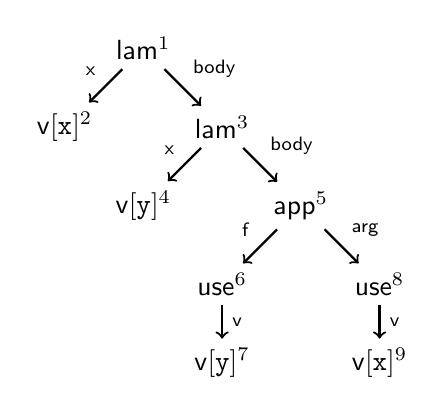
\begin{tikzpicture}
\node(r) at (0,0) {\textsf{lam}$^1$};
    \node(r1) at (-1,-1) {\textsf{v}[\texttt{x}]$^2$};
    \node(r2) at (1,-1) {\textsf{lam}$^3$};
        \node(r21) at (0,-2) {\textsf{v}[\texttt{y}]$^4$};
        \node(r22) at (2,-2) {\textsf{app}$^5$};
            \node(r221) at (1,-3) {\textsf{use}$^6$};
                \node(r2211) at (1,-4) {\textsf{v}[\texttt{y}]$^7$};
            \node(r222) at (3,-3) {\textsf{use}$^8$};
                \node(r2221) at (3,-4) {\textsf{v}[\texttt{x}]$^9$};
\draw [thick,->] (r)    -- node[above left]  {\scriptsize\textsf{x}}    (r1);
\draw [thick,->] (r)    -- node[above right] {\scriptsize\textsf{body}} (r2);
\draw [thick,->] (r2)   -- node[above left]  {\scriptsize\textsf{x}}    (r21);
\draw [thick,->] (r2)   -- node[above right] {\scriptsize\textsf{body}} (r22);
\draw [thick,->] (r22)  -- node[above left]  {\scriptsize\textsf{f}}    (r221);
\draw [thick,->] (r22)  -- node[above right] {\scriptsize\textsf{arg}}  (r222);
\draw [thick,->] (r221) -- node[right]       {\scriptsize\textsf{v}}    (r2211);
\draw [thick,->] (r222) -- node[right]       {\scriptsize\textsf{v}}    (r2221);
\end{tikzpicture}

A more familiar rendering of this tree would not have labels on each edge, but the visual ordering left-to-right would indicate which child is which.
By coloring each edge with a label, we make this idea mathematically rigorous.
In addition, drawing an AST need not be restricted to particular geometric forms.
This drawing is exactly the same tree as the one above, as is usual for general graphs:
\newline
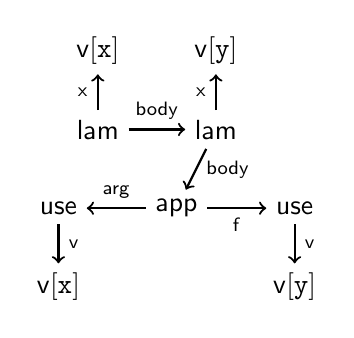
\begin{tikzpicture}
\node(r) at (-1,0) {\textsf{lam}};
    \node(r1) at (-1,1) {\textsf{v}[\texttt{x}]};
    \node(r2) at (0.5,0) {\textsf{lam}};
        \node(r21) at (0.5,1) {\textsf{v}[\texttt{y}]};
        \node(r22) at (0,-1) {\textsf{app}};
            \node(r221) at (1.5,-1) {\textsf{use}};
                \node(r2211) at (1.5,-2) {\textsf{v}[\texttt{y}]};
            \node(r222) at (-1.5,-1) {\textsf{use}};
                \node(r2221) at (-1.5,-2) {\textsf{v}[\texttt{x}]};
\draw [thick,->] (r)    -- node[left]        {\scriptsize\textsf{x}}    (r1);
\draw [thick,->] (r)    -- node[above]       {\scriptsize\textsf{body}} (r2);
\draw [thick,->] (r2)   -- node[left]        {\scriptsize\textsf{x}}    (r21);
\draw [thick,->] (r2)   -- node[right]       {\scriptsize\textsf{body}} (r22);
\draw [thick,->] (r22)  -- node[below]       {\scriptsize\textsf{f}}    (r221);
\draw [thick,->] (r22)  -- node[above]       {\scriptsize\textsf{arg}}  (r222);
\draw [thick,->] (r221) -- node[right]       {\scriptsize\textsf{v}}    (r2211);
\draw [thick,->] (r222) -- node[right]       {\scriptsize\textsf{v}}    (r2221);
\end{tikzpicture}
\newline
I'll try to contain myself.


\subsection{Binding Grammars and Trees}

Intuition tells us that binding is an additional layer atop syntax, and that is exactly how we will represent it.
An abstract binding tree (ABT) $G = \langle G_0, B \rangle$ is an abstract syntax tree $G_0$ augmented with an additional set of binding edges $B$.
If there is a binding edge from $v$ to $v'$, we write $v \dashedrightarrow v'$.
Note that these binding edges are not colored.
The binding edges in an ABT are subject to the restrictions:
\begin{enumerate}
    \item $\forall v_1 \dashedrightarrow v_2 \in G.\,
            \mathsf{col}(v_1) = \mathsf{col}(v_2) \land
            \nexists v' \in G. v_1 \to v' \lor v_2 \to v'$

            Binding edges only connect leaf vertices of the same color.
    \item $\forall v_u \dashedrightarrow v_d \in G.\,
            (\nexists v.\, v \dashedrightarrow v_u) \land
            (\nexists v. v_d \dashedrightarrow v)$

            A vertex can have only incoming or outgoing binding edges, but not both.

    \item $\forall v \in G.\,
            \forall v \dashedrightarrow v_1, v \dashedrightarrow v_2.
            v_1 = v_2$

            A vertex has at most one binding outgoing edge.
\end{enumerate}

The upshot of these definitions is that we can draw an ABT, say of $\fn x.\,\fn x.\, x\;x$, with an intuitive diagram:
\newline
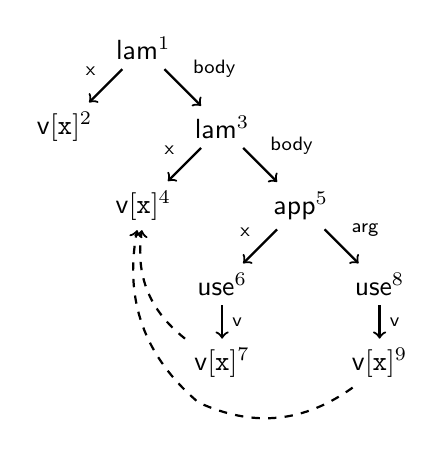
\begin{tikzpicture}
\node(r) at (0,0) {\textsf{lam}$^1$};
    \node(r1) at (-1,-1) {\textsf{v}[\texttt{x}]$^2$};
    \node(r2) at (1,-1) {\textsf{lam}$^3$};
        \node(r21) at (0,-2) {\textsf{v}[\texttt{x}]$^4$};
        \node(r22) at (2,-2) {\textsf{app}$^5$};
            \node(r221) at (1,-3) {\textsf{use}$^6$};
                \node(r2211) at (1,-4) {\textsf{v}[\texttt{x}]$^7$};
            \node(r222) at (3,-3) {\textsf{use}$^8$};
                \node(r2221) at (3,-4) {\textsf{v}[\texttt{x}]$^9$};
\draw [thick,->] (r)    -- node[above left]  {\scriptsize\textsf{x}}    (r1);
\draw [thick,->] (r)    -- node[above right] {\scriptsize\textsf{body}} (r2);
\draw [thick,->] (r2)   -- node[above left]  {\scriptsize\textsf{x}}    (r21);
\draw [thick,->] (r2)   -- node[above right] {\scriptsize\textsf{body}} (r22);
\draw [thick,->] (r22)  -- node[above left]  {\scriptsize\textsf{x}}    (r221);
\draw [thick,->] (r22)  -- node[above right] {\scriptsize\textsf{arg}}  (r222);
\draw [thick,->] (r221) -- node[right]       {\scriptsize\textsf{v}}    (r2211);
\draw [thick,->] (r222) -- node[right]       {\scriptsize\textsf{v}}    (r2221);
\draw [thick,dashed,->] (r2211) to[bend left] (r21);
\draw [thick,dashed,->] (r2221) to[bend left] (0.7,-4.5) to[bend left] (r21);
\end{tikzpicture}
\newline
Notice that the corresponding AST is obtained simply by erasing binding edges.
One might ask if it is possible to go in the opposite direction, from an AST to a grammatical ABT?
Indeed, this is required for scope analysis, so it had better be possible.
% Shortly, we will manually define just such a binding inferencer in the language of out ASTs and ABTs.
% First, I would like to point out that an AST may have several grammatical ABTs, but there is a natural restriction our inferencer should satisfy.
% If $G$ is an ABT, then there should exist some $G'$ obtained by $\alpha$-renaming $G$ such that if $G'_0$ is the AST obtained by erasing binding edges from $G'$, then our binding inferencer should recover $G'$ from $G'_0$.


Rather than examine the ABTs of the lambda calculus, which is easily handled by Martin-L\"of's presentation of ABTs, let's examine a somewhat tricker calculus.
Namely, let's extend the lambda calculus with tuples and patterns (including pair-destructuring and view patterns), the syntax of which is given below, along with some operator and label names for later use.

\begin{tabular}{rclcl}
$x$ & $\in$ & $\mathcal{X}$ &$\quad$& $\mathsf{v}[x]$ \\
$e$ & $::=$ & $x$ && $\mathsf{use}(\mathsf{x})$ \\
& $\mid$ & $\fn p.\,e$ && $\mathsf{lam}(\mathsf{p, body})$ \\
& $\mid$ & $e\;e$ && $\mathsf{app}(\mathsf{f, arg})$ \\
& $\mid$ & $(e, \ldots, e)$ && $\mathsf{tupE}[n](1, \ldots, n)$ \\
$p$ & $::=$ & $x$ && $\mathsf{def}(\mathsf{x})$ \\
& $\mid$ & $(p, \ldots, p)$ && $\mathsf{tupP}[n](1, \ldots, n)$ \\
& $\mid$ & $e \to p$ && $\mathsf{viewP}(\mathsf{f, p})$ \\
\end{tabular}

The key idea is that where a scope is introduced, intendedly-binding names are gathered from some sub-terms, then they are distributed to sub-terms for intendedly-bound names to target.
For the former operation we use the judgment on a vertex $v \vdash \Gamma$, which we call the name gatherer.
The resulting environment $\Gamma$ is a finite map from operator to vertex.
For the latter, we use the judgment on a vertex $\Gamma \vdash v \leadsto B$, which we call the name distributor.
The result, $B$, is a set of binding edges.
For an AST $G$, we will infer an ABT $\langle G, B \rangle$ when $\emptyset \vdash \overset{\downarrow}v \leadsto B$.

Rather than write these rules directly, we can reduce the apparent number of premises by exploiting the fact that each rule will be vertex-directed and ``syntax''-directed (in the sense that the coloring of the vertex under study drives the inference).
In the conclusions of rules for both gatherers and distributors, we will write in place of the vertex metavariable, $v$, only a coloring with the meaning that the rule only applies to vertices with that coloring.
Since this will remove our ability to bind a name for the vertex under study, we will conventionally use $v$ not as a metavariable, but as the name for that vertex.

\begin{figure}[H]
\centering
    % \begin{subfigure}[t]{0.3\textwidth}
    % \centering
    $$
        \AxiomC{}
        \UnaryInfC{$\mathsf{v}[x] \vdash \{\mathsf{v}[x] \mapsto v\}$}
        \DisplayProof$$
    $$
        \AxiomC{$v(\mathsf{x}) \vdash B$}
        \UnaryInfC{$\mathsf{def} \vdash B$}
        \DisplayProof$$
    $$
        \AxiomC{$v(i) \vdash B_i$}
        \UnaryInfC{$\mathsf{tupP}[n] \vdash \bigoplus\limits_{i = 1}^n\,B_i$}
        \DisplayProof$$
    $$
        \AxiomC{$v(\mathsf{p}) \vdash B$}
        \UnaryInfC{$\mathsf{viewP} \vdash B$}
        \DisplayProof$$
    % \end{subfigure}
    % \begin{subfigure}[t]{0.3\textwidth}
    % \centering
    \vspace{0.5cm}
    $$
        \AxiomC{$\Gamma(\mathsf{v}[x]) = v'$}
        \UnaryInfC{$\Gamma \vdash \mathsf{v}[x] \leadsto \{v \dashedrightarrow v'\}$}
        \DisplayProof$$
    $$
        \AxiomC{$\Gamma \vdash v(\mathsf{x}) \leadsto B$}
        \UnaryInfC{$\Gamma \vdash \mathsf{use} \leadsto B$}
        \DisplayProof$$
    $$
        \AxiomC{$v(\mathsf{p}) \vdash \Gamma'$}
        \AxiomC{$\Gamma,\Gamma' \vdash v(\mathsf{p}) \leadsto B_p$}
        \AxiomC{$\Gamma,\Gamma' \vdash v(\mathsf{body}) \leadsto B_b$}
        \TrinaryInfC{$\Gamma \vdash \mathsf{lam} \leadsto B_p \cup B_b$}
        \DisplayProof$$
    $$
        \AxiomC{$\Gamma \vdash v(\mathsf{f}) \leadsto B_1$}
        \AxiomC{$\Gamma \vdash v(\mathsf{arg}) \leadsto B_2$}
        \BinaryInfC{$\Gamma \vdash \mathsf{app} \leadsto B_1 \cup B_2$}
        \DisplayProof$$
    $$
        \AxiomC{$\Gamma \vdash v(i) \leadsto B_i$}
        \UnaryInfC{$\Gamma \vdash \mathsf{tupE}[n] \leadsto \bigcup\limits_{i = 1}^n\,B_i$}
        \DisplayProof$$
    $$
        \AxiomC{}
        \UnaryInfC{$\Gamma \vdash \mathsf{def} \leadsto \emptyset$}
        \DisplayProof$$
    $$
        \AxiomC{$\Gamma \vdash v(i) \leadsto B_i$}
        \UnaryInfC{$\Gamma \vdash \mathsf{tupP}[n] \leadsto \bigcup\limits_{i=1}^n\,B_i$}
        \DisplayProof$$
    $$
        \AxiomC{$\Gamma \vdash v(\mathsf{f}) \leadsto B_1$}
        \AxiomC{$\Gamma \vdash v(\mathsf{p}) \leadsto B_2$}
        \BinaryInfC{$\Gamma \vdash \mathsf{viewP} \leadsto B_1 \cup B_2$}
        \DisplayProof$$
    % \end{subfigure}
\end{figure}

Even after trimming down the notation, these rules are still verbose, but at least they follow a very regular pattern.
For $\mathsf{v}[x]$, the rules do the only sensible thing.
For the other gathering judgments, each pattern operator simply combines the results from its pattern sub-trees; in this case, the combination is $\oplus$ (which is union, except where the operands are not disjoint, in which case it is undefined).
Most of the other distributing judgments simply recurse into sub-trees and combine the resulting sets of binding edges with plain union.
The only exceptions are the rules for \textsf{lam}, and \textsf{def}, but even then, the interesting each of these rules is only a portion of the whole rule.
In particular, all distributing judgments gather sub-terms from a set of children, then recurse into children with environments constructed from the initial and gathered environments, and finally combine the resulting binding edges with plain union.
In most distributing rules, the set to gather from is empty, and the new environments are simply the initial environment.
The \textsf{lam, def} rules are interesting only in that the set to gather from is $\{\mathsf{p}\}, \emptyset$ respectively, and the new environments are $\{\mathsf{p} \mapsto \Gamma,\Gamma'; \mathsf{body} \mapsto \Gamma,\Gamma'\}, \emptyset$.



We would much rather write the following, or perhaps something even less heavyweight.
Here, the symbols before the arrow and in the numerators bind over the denominators for each operator.
Those in the denominator are the results of name-gathering premises, whereas those in the denominator set up a new environments in which the recursive binding-gathering premises operate.
\newline
\begin{tabular}{rclcl}
$x$ & $\in$ & $\mathcal{X}$ &$\quad$& \\
$e$ & $::=$ & $x$ &&  \\
& $\mid$ & $\fn p.\,e$ && $\Gamma \to \fn \frac{\Gamma'}{\Gamma,\Gamma'}p.\, \frac{}{\Gamma,\Gamma'}e$ \\
& $\mid$ & $e\;e$ &&  \\
& $\mid$ & $(e, \ldots, e)$ &&  \\
$p$ & $::=$ & $x$ && $\Gamma \to \frac{}{\emptyset}x$ \\
& $\mid$ & $(p, \ldots, p)$ &&  \\
& $\mid$ & $e \to p$ &&  \\
\end{tabular}
\newline
The trick now is to develop a rigorous method by which the boring parts of the binding inference rules can be recovered from such a description.
To do so, we will first need to make these notations for binding rigorous.


\subsection{General Patterns of Binding Inference}

Given an abstract grammar, we can define a binding grammar is a three-way partition of the sorts and a binding inferencer.
The partitioning $S = N \oplus D \oplus U$ splits the sorts $S$ of the abstract grammar into disjoint sets of name sorts $V$, definition sorts $D$, and usage sorts $U$.
Additionally, the $N$ partition should only contain colors of leaf nodes.
A binding inferencer $F$ is a pair of functions $\langle F_\uparrow, F_\downarrow \rangle$.
These functions are called the upwards and downwards name flow respectively.
Before describing these in detail, we will need a function similar to $\Ell(o) = \mathsf{dom}(V_\downarrow(c))$, which restricts the label enumeration to those which point towards vertices with operators not of usage sort: $\Ell'(o) = \{\ell \in \Ell(o) \mid V_\uparrow(o)(\ell) \nin U\}$.
Both name flows are curried dependent functions, so let's examine each individually.

The idea behind the upwards name flow is to specify a method for gathering names by combining environments from the names gathered from sub-terms.
Its first argument is an definition operator $o \in D$, and then returns a gathering function.
The gathering function takes a finite map of environments indexed by the labels of that operator's child edge labels and returns a new environment.
The gathering function may be partial; this allows for derivations to fail based on some context-sensitive requirements (such as binders in patterns of the same scope must be disjoint, as in Haskell pattern-matching).
This is summarized by:
    $$F_\uparrow : \Pi\,o{:}D \to (\Ell(o) \mapsto \Gamma) \nrightarrow \Gamma$$

The idea behind the downwards name flow is to specify a method for distributing names from a scoping term to its sub-terms.
It takes two arguments first: an operator and a label for an outward edge from that operator.
It then returns a distribution function which is a total function from a number of environments to another environment.
The input environments are for the initial environment, and a finite map describing the environments gathered from subterms.
In summary:
    $$F_\downarrow : \Pi\,o{:}N^\mathsf{C} \times L(o) \to (\Gamma \times (\Ell'(o) \mapsto \Gamma)) \to \Gamma$$

We now present a system of natural deduction which can be used for any binding grammar.
Because these rules often have access to a vertex, but must apply a function to the operator coloring that vertex, it will be useful to abuse notation to reduce the line noise.
Thus, we will write $f(v)$ for $f(\mathsf{col}(v))$ where no ambiguity would result.
Also note that we will have need of finite map comprehension $\{x \mapsto y \mid x \in S\}$, which strictly speaking is exactly set comprehension, but may feel different , and notation is not as standard.

\begin{figure}[H]
\centering
$$
    \AxiomC{$V_\uparrow(v) \in N$}
    \UnaryInfC{$v \vdash \{\mathsf{col}(v) \mapsto v\}$}
    \DisplayProof$$
$$
    \AxiomC{$V_\uparrow(v) \in D$}
    \AxiomC{$\overline{v(\ell) \vdash \Gamma_\ell}^{\ell \in \Ell'(v)}$}
    \BinaryInfC{$v \vdash F_\uparrow(v)(\{\ell \mapsto \Gamma_\ell \mid \ell \in \Ell'(v)\})$}
    \DisplayProof$$
$$
    \AxiomC{$V_\uparrow(v) \in N$}
    \AxiomC{$\Gamma(\mathsf{col}(v)) = v'$}
    \BinaryInfC{$\Gamma \vdash v \leadsto \{v \dashedrightarrow v'\}$}
    \DisplayProof$$

$$
    \AxiomC{$V_\uparrow(v) \nin N$}
    \AxiomC{$\overline{v(\ell') \vdash \Gamma_{\ell'}}^{\ell' \in \Ell'(v)}$}
    \AxiomC{$\overline{F_\downarrow(v, \ell)(\Gamma, \{\ell' \mapsto \Gamma_{\ell'} \mid \ell' \in \Ell'\}) \vdash v(\ell) \leadsto B_\ell}^{\ell \in \Ell(v)}$}
    \TrinaryInfC{$\Gamma \vdash v \leadsto \bigcup\limits_{\ell \in \Ell(v)} B_\ell$}
    \DisplayProof$$
\end{figure}

The first thing to note about these rules is that they are driven by which partition the vertex's operator falls into.
Let's look first at the rules relating to name sorts (where the premises include $V_\uparrow(v) \in N$).
The gathering rule for name sorts constructs a singleton environment, and the name rule looks up a vertex from that environment; the link between the two is by the operator, thus satisfying our requirement 1 of ABTs.
The other rules serve to transport each gathered binding to lookup sites.

The gathering rule for usage sorts recurses into subterms to build up a dictionary of environments $\{\ell' \mapsto \Gamma_{\ell'} \mid \ell' \in \Ell'\}$.
Once these environments are obtained, they are fed into the appropriate upwards-flow function $F_\uparrow(v)$.
Note that the recursion only enters non-definition-sorted subterms $\Ell'(v)$; that is, definition-sorts are never asked to gather variables.
As such, there is no gathering rule for definition sorts.
Further, since $F_\uparrow(v)$ is a partial function, it may fail to produce a gathered environment; in such cases, the rule is not satisfied.

The most imposing rule is that for distributing for non-name sorts, but it is actually straightforward when broken down.
First, environments are gathered from subterms, giving a dictionary of environments $\{\ell' \mapsto \Gamma_{\ell'} \mid \ell' \in \Ell'\}$ just as before.
Then, for each subterm, the downwards flow is consulted to yield a distribution function $F_\downarrow(v, \ell)$.
The distribution function is called with the initial environment and the dictionary gathered in the first step $(\Gamma, \{\ell' \mapsto \Gamma_{\ell'} \mid \ell' \in \Ell'\})$.
This gives a binging edge set $B_\ell$ for each child node, all of which are unioned together.


To illustrate, let's return to our example of the lambda-calculus with tuples and patterns.
The sorts are partitioned as $S = \langle N, D, U \rangle = \langle \{\mathsf{var}\}, \{\mathsf{pat}\}, \{\mathsf{expr}\} \rangle$.
We can then define the upward flow:
\begin{align*}
F_\uparrow(\mathsf{def})(\{\mathsf{v}\mapsto\Gamma\}) =\;& \Gamma \\
F_\uparrow(\mathsf{tupP}[n])(\{\overline{i\mapsto\Gamma_i}\}) =\;& \bigoplus\limits_{i = 1}^n\Gamma_i \\
F_\uparrow(\mathsf{viewP})(\{\mathsf{p}\mapsto\Gamma\}) =\;& \Gamma \\
\end{align*}
and the downward flow:
\begin{align*}
F_\downarrow(\mathsf{use}, \mathsf{v})(\Gamma, \{\}) =\;& \Gamma \\
F_\downarrow(\mathsf{lam}, \_)(\Gamma, \{\mathsf{p} \mapsto \Gamma'\}) =\;& \Gamma,\Gamma' \\
F_\downarrow(\mathsf{app}, \_)(\Gamma, \{\}) =\;& \Gamma \\
F_\downarrow(\mathsf{tupE}[n], \_)(\Gamma, \{\}) =\;& \Gamma \\
F_\downarrow(\mathsf{use}, \_)(\_, \_) =\;& \emptyset \\
F_\downarrow(\mathsf{tupP}[n], i)(\Gamma, \_) =\;& \Gamma \\
F_\downarrow(\mathsf{viewP}, \_)(\Gamma, \_) =\;& \Gamma \\
\end{align*}
So far, this definition is just as boring, if slightly more concise, than 
However, we are now ready to formalize the boring parts we informally identified earlier.


Let $\odot$ be a commutative (possibly) partial function over environments.
We will say that $F_0 = \langle F_{0\uparrow}, F_{0\downarrow} \rangle$ is a default binding inferencer.
Then
\begin{align*}
F_{0\uparrow}^\odot(o)(\{\overline{\ell \mapsto \Gamma_\ell}\}) =\;& \bigodot\limits_\ell \Gamma_\ell \\
F_{0\downarrow}(o, \ell)(\Gamma, \harpvec{\Gamma'}) =\;& \Gamma \\
\end{align*}
Although I personally prefer using the disjoint-by-precondition union for calculi, there is no theoretical reason a different operator could be used, which is why I have left $\odot$ as a parameter.

For our extended lambda calculus, we can now reduce the definition of binding inference to a meager few declarations.
First, we have the sort partition as above.
Then, the binding inferencer is $F_0$ using $\oplus$, except for the following two cases:
\begin{align*}
F_\downarrow(\mathsf{lam}, \_)(\Gamma, \{\mathsf{p} \mapsto \Gamma'\}) =\;& \Gamma,\Gamma' \\
F_\downarrow(\mathsf{use}, \_)(\_, \_) =\;& \emptyset \\
\end{align*}
There will of course be common patterns even in these exceptions, but let's first introduce a convenient notation for this prose.

To the side of each BNF-style production for an abstract grammar, there may be a binding specification written.
If no such specification is given, then use the default rule for this production.
Otherwise, a binding specification takes the form of a name for the initial environment, then an arrow, then the BNF-style rule again except that each metavariable is preceded by a fraction(-sort-of-looking-thing).
The numerator of this fraction introduces a name for the set of gathered names from that child.
The denominator is the body of distributor function for that child.
Where a denominator is not given, use the default distributor function.
Where there is no gathered set for a subterm, leave the numerator blank.

The name sorts are generally obvious, so need not be explicitly given, even in complex calculi.
The partition between definition and usage sorts is slightly tricker, but can be recovered by identifying metavariables that bind a gathered name set: those that do are for definition sorts, whereas the others are for usage sorts.
Finally, the parameter $\odot$ should strictly be stated in text, but I expect it will be $\oplus$ nearly all of the time.

Given this, we now know how to interpret our proposed notation from above into the more explicit binding inference system.
However, there are still a few repeated patterns in common calculi that could be omitted.
If the binding for initial environment (including the arrow) is left out, then each (non-blank) numerator can omit the $\Gamma,\cdot$ without a change in meaning.
Similarly, appearances of names will often require the empty set as the denominator; for this, another notation might be advisable.
I haven't settled on one myself, but perhaps the following suggestion is sufficient:

\begin{tabular}{rclcl}
$x$ & $\in$ & $\mathcal{X}$ &$\quad$& \\
$e$ & $::=$ & $x$ &&  \\
& $\mid$ & $\fn p.\,e$ && $\fn \frac{\Gamma'}{\Gamma'}p.\, \frac{}{\Gamma'}e$ \\
& $\mid$ & $e\;e$ &&  \\
& $\mid$ & $(e, \ldots, e)$ &&  \\
$p$ & $::=$ & $x$ && $\underset{\dasheduparrow}x$ \\
& $\mid$ & $(p, \ldots, p)$ &&  \\
& $\mid$ & $e \to p$ &&  \\
\end{tabular}

The reader may have noted that there is no facility in this notation to override the name gathering process.
I have yet to encounter a calculus that requires this, but just in case, I propose to prefix the initial environment with a left arrow pointing to an expression for the body of the combination.

\subsection{Extensions}

TODO: multiple environments in judgements (use tuples of environments everywhere environments \textit{simpliciter} are used in the long-form; separate by semicolon in the short notation).
The default rule for gathering names will have to be adding them to everything; for looking up, prefer the latest.

\subsection{Free Variables, Hygienic Substitution, $\alpha$-renaming}

TODO

FIXME: free variables seem easy: any name-sorted vertices without a binding edge, but then what about binders that go unused?
Perhaps a judgement $v \vdash \{\harpvec{v'}\} \mathsf{ binders}$ which is true whenever $v \vdash \{\overline{o \mapsto v'}\}$ for any operators $\harpvec o$.
Then, free variables are given by the operators coloring the set of binding edge-less name-sorted vertices minus binders from the judgment.
In fact, I should have a judgment (say to $\gamma \vdash v \leadsto_\mathsf{fv} B$) which collects free variables;
indeed, it might be useful to add vertices to the graph which target and are targeted by binding edges.

\section{Example Binding Calculi}

Applied lambda calculi:
\newline
\begin{tabular}{rclcl}
$x$ & $\in$ & $\mathcal{X}$ \\
$c$ & $\in$ & $\mathcal{C}$ &$\quad$& \\
$e$ & $::=$ & $x$ &&  \\
& $\mid$ & $\fn x.\,e$ && $\fn \frac{\Gamma'}{}x.\, \frac{}{\Gamma'}e$ \\
& $\mid$ & $e\;e$ &&  \\
& $\mid$ & $c$ &&  \\
\end{tabular}

The pi calculus
\newline
\begin{tabular}{rclcl}
$x$ & $\in$ & $\mathcal{X}$ &$\quad$& \\
$P$ & $::=$ & $\nu\:\!x.\,P$
    && $\nu\:\!\frac{\Gamma'}{}x.\,\frac{}{\Gamma'}P$ \\
& $\mid$ & $x(x).P$
    && $x(\frac{\Gamma'}{}x)\frac{}{\Gamma'}P$ \\
& $\mid$ & $\bar x\langle x \rangle.P$ \\
& $\mid$ & $0$ \\
& $\mid$ & $P | P$ \\
& $\mid$ & $!P$ 
\end{tabular}

A miniature (untyped) C-like language with a scope-restriction block:
\newline
\begin{tabular}{rclcl}
$x$ & $\in$ & $\mathcal{X}$ &$\quad$& \\
$D$ & $::=$ & $d_1 \ldots d_n$
    && $\bigcup_i\Delta_i;\emptyset \leftarrow
    \Delta;\; \to \frac{\Delta_1;}{}d_1 \ldots \frac{\Delta_n;}{\Delta_1, \ldots, \Delta_{n-1};}d_n$ \\
$d$ & $::=$ & $\mathsf{decl}\;x$
    && $\Delta';\emptyset \leftarrow \mathsf{decl}\;\frac{\Delta';}{}x$ \\
& $\mid$ & $\mathsf{def}\;x(x_1, \ldots, x_n){:}\;S$
    && $\Delta';\emptyset \leftarrow \;;\Gamma \to
    \mathsf{def}\;\frac{\Delta';}{}x(\frac{;\Gamma_1}{}x_1, \ldots, \frac{;\Gamma_n}{}x_n){:}\;\frac{}{\Delta';\Gamma_1,\ldots,\Gamma_n}S$ \\
& $\mid$ & $\mathsf{var}\;x = e$
    && $\Delta';\emptyset \leftarrow \mathsf{var}\;\frac{\Delta';}{}x = \frac{}{}e$ \\
$S$ & $::=$ & $s_1; \ldots; s_n$
    && $\frac{;\Gamma_1}{}d_1 \ldots \frac{;\Gamma_n}{;\Gamma_1, \ldots, \Gamma_{n-1}}d_n$ \\
$s$ & $::=$ & $\mathsf{var}\;x = e$
    && $\emptyset;\Gamma' \leftarrow \mathsf{var}\;\frac{;\Gamma'}{}x = e$ \\
& $\mid$ & $x = e$ \\
& $\mid$ & $\mathsf{return}\;e$ \\
& $\mid$ & $\mathsf{only}\;(x_1, \ldots, x_n)\;\{S\}$
    && $;\Gamma \to \mathsf{only}\;(\frac{;\Gamma_1}{}x_1, \ldots, \frac{;\Gamma_n}{}x_n)\;\{\frac{}{;\bigcup_i \Gamma_i}S\}$ \\
$e$ & $::=$ & $x$ &&  \\
& $\mid$ & $e(e_1, \ldots, e_n)$ &&  \\
\end{tabular}
\newline
If a name sort is preceded with a fraction and only some of the environment tuple are given a name, the name only gets added to the appearing tuple elements.

A predicate logic with quantification bounded by arbitrary formulae:
\newline
\begin{tabular}{rclcl}
$x$ & $\in$ & $\mathcal{X}$ &$\quad$& \\
$f$ & $\in$ & $\mathcal{F}$ \\
$\otimes$ & $\in$ & $\{\to, \land, \lor\}$ \\
$\mathfrak{Q}$ & $\in$ & $\{\forall, \exists\}$ \\
$P$ & $::=$ & $x$ && \\
& $\mid$ & $f(P_1, \ldots, P_n)$ &&  \\
& $\mid$ & $\neg P$ &&  \\
& $\mid$ & $P \otimes P$ &&  \\
& $\mid$ & $\mathfrak{Q} x_1,\ldots, x_n.\,P$
    && $\forall \frac{\Gamma_1}{}x_1,\ldots, \frac{\Gamma_n}{}x_n.\,\frac{}{\Gamma_1,\ldots,\Gamma_n}P$ \\
& $\mid$ & $\mathfrak{Q} P.\,P$
    && $\Gamma \to \forall \frac{\Gamma'}{}P.\,\frac{}{\Gamma,(\Gamma' - \Gamma)}P$ \\
\end{tabular}





\end{document}






Let $G$ be a set of grammatical categories and $N$ be a set of node constructors.
Then a syntax $\mathcal{L}$ is a triple $\langle G, N, ar \rangle$, where $ar$ is an arity function ranging over node constructors.
The exact form of the arity function will depend on the uses to which the syntax will be put.
We will eventually come to abstract binding trees, but first, we will examine the more familiar case of abstract syntax trees.

$$
\mathtt{Syntax} \equiv
    \lambda ar^{\star \to \star}.
    \Sigma gcat^\star \times
    \Sigma ctor^\star \times
    (ctor \to ar\;gcat)
$$



For abstract syntax trees, the arity describes the grammatical category of a syntax node, and whether that node is terminal or non terminal.
When the node is terminal, it also describes the set from which that terminal is to be drawn.
Alternately, when the node is non-terminal, it also describes the number and grammatical categories of its immediate subterms.

$$ \mathtt{CFArity} \equiv
    \lambda g^{\star}.
    g \times
    (\star + \mathtt{List}\;g)
$$

$$
\mathtt{AST} \equiv \mathtt{Syntax}\;\mathtt{CFArity}
$$

$$
\mathtt{CFTerm} \equiv
    \lambda l^{\mathtt{AST}}.
    \lambda g^{l.1}.
    \Sigma ctor^{l.2} \times
    (g = (l.3\;l\;ctor).1) \times
    \mathtt{subterms}\;l\;ctor
$$
where
\begin{align*}
\mathtt{subterms} \equiv
    \lambda l^\mathtt{AST}.
    \lambda ctor^{l.2}.
    \textsf{case }(l.3\;ctor).2\textsf{ of } \{ \\
        \iota_1\;\alpha \to \alpha \\
        \iota_2\;gs \to \mathtt{Tuple}\;(\mathtt{CFTerm}\;l \mathbin{\texttt{<\$>}} gs) \\
    \}
        % subterms = λ(l : Language, ctor : Ctor l).
        %     case ctor of
        %         { ι_1 α → α
        %         , ι_2 gcats → Tuple (Term l <$> gcats)
        %         }
\end{align*}
